\documentclass[12pt,addpoints]{exam}
%\usepackage{enumitem}
\usepackage{amsfonts,amssymb,amsmath, amsthm}
\usepackage{graphicx}
\usepackage{systeme}
\usepackage{pgf,tikz,pgfplots}
\pgfplotsset{compat=1.15}
\usepgfplotslibrary{fillbetween}
\usepackage{mathrsfs}
\usetikzlibrary{arrows}
\usetikzlibrary{calc}
\usepackage{geometry}
\geometry{
	a4paper,
	total={170mm,257mm},
	left=15mm,
	right=15mm,
	bottom=20mm,
	top=15mm,
}
\date{November, 2023}
\pagestyle{headandfoot}
%\firstpageheadrule
\runningheader{1st Quarter Final Examination}{}{Page \thepage\ of \numpages}
\runningheadrule
\firstpagefooter{}{}{}
\runningfooter{By Aaron G.K.}{}{Page \thepage\ of \numpages}
\begin{document}
	\title{St John Baptist De La Salle Catholic School, Addis Ababa\\
		\large Grade 11 Physics Final Examination \\
		$1^\text{st}$ Quarter}
	\maketitle
	\begin{center}
		\fbox{\fbox{\parbox{6in}{\centering
					Notes, and use of other aids is \textbf{NOT} allowed.  Read all directions carefully and \textbf{write your answers in the answer sheet}.  To receive full credit, you must show all of your work. \textbf{USE OF CALCULATORS IS ALLOWED}.
	}}}	\end{center}
	{Name:\underline{\hspace{2in}}\text{     }{Roll Number:\underline{\hspace{0.5in}}\text{     }{Section:\underline{\hspace{0.3in}}{Time Allowed: \bf{1.5 hours}}
				\subsection*{Multiple Choice Questions} 
				\subsubsection*{Choose the BEST answer out of the given options and mark your answers in the answer box on the last page}\textit{(1 points each)} 
				\begin{questions}
					\question Which of the following research repositories is NOT free access? \\
					\begin{oneparchoices}
						\choice The arXiv
						\choice Nature Journal
						\choice NASA ADS \\
						\choice Inspire HEP
						\choice None of the above
					\end{oneparchoices}	\\
					\textbf{Answer: B}
					\question Which of the following physics coalitions detected the speed of gravitational waves to be $299,792,858m/s$? \\
					\begin{oneparchoices}
						\choice WMAP collaboration
						\choice LISA collaboration 
						\choice CERN Collaboration \\
						\choice LIGO collaboration
						\choice None of the above
					\end{oneparchoices}\\
					\textbf{Answer: D}
					\question  The vectors $\vec{a}$, $\vec{b}$, and $\vec{c}$ are related by $\vec{c}$ = $\vec{b}-\vec{a}$. Which diagram below illustrates this
					relationship?
					\begin{center}
						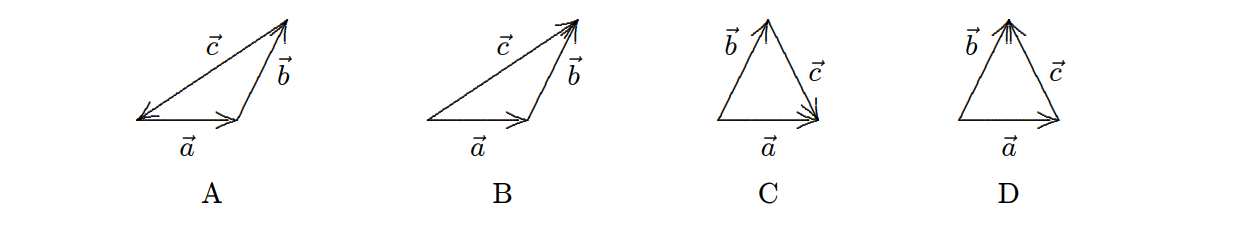
\includegraphics[scale=0.4]{vecs.png}
					\end{center}
					\textbf{Answer: D}
					\question A vector of magnitude 3 CANNOT be added to a vector of magnitude 4 so that the magnitude of the resultant is:\\
					\begin{oneparchoices}
						\choice 0
						\choice 1
						\choice 3
						\choice 7
						\choice 5
					\end{oneparchoices}
					\\
					\textbf{Answer: A}
					\question If $|\vec{A}+\vec{B}|=A^2+B^2$, then which of the following is true?
					\begin{choices}
						\choice $\vec{A}$ and $\vec{B}$ must be parallel (\textit{and in the same direction})
						\choice $\vec{A}$ and $\vec{B}$ must be parallel in the opposite direction(\textit{are anti-parallel})
						\choice Either $\vec{A}$ or $\vec{B}$ are zero.
						\choice The angle between $\vec{A}$ and $\vec{B}$ is $\dfrac{\pi}{2}$
						\choice None of the above is true.
					\end{choices}
					\textbf{Answer: D}
					\question Four vectors ($\vec{A}$, $\vec{B}$, $\vec{C}$, $\vec{D}$) all have the same magnitude. The angle $\theta$ between adjacent vectors
					is 45$^\circ$ as shown. The correct vector equation is
					\begin{center}
						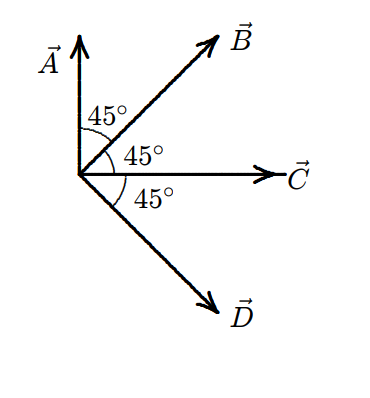
\includegraphics[scale=0.4]{vecs2.png}
					\end{center} 
					\begin{oneparchoices}
						\choice $\vec{A}-\vec{B}-\vec{C}+\vec{D}=0$
						\choice $\vec{A}+\vec{B}+\vec{C}+\vec{D}=0$ 
						\choice $\vec{B}+\vec{D}-\sqrt{2}\vec C=0$
						\choice $\vec{A}+\vec{B}=\vec{B}+\vec{D}=0$
						\choice $\dfrac{\vec{A}+\vec{C}}{\sqrt{2}}=-\vec{B}$	
					\end{oneparchoices}
					\\
					\textbf{Answer: C}
					\question The angle between the vector $\vec{A}=-2.5m\hat i+4.5m\hat j$ and the positive x-axis is? \\ 
					\begin{oneparchoices}
						\choice $29^\circ$
						\choice $39^\circ$
						\choice $119^\circ$
						\choice $70^\circ$
						\choice $61^\circ$
					\end{oneparchoices}
					\\ \textbf{Answer: C}
					\question A vector has a component of 10 m in the +x direction, a component of 10 m in the +y direction,
					and a component of 5 m in the +z direction. The magnitude of this vector is: \\
					\begin{oneparchoices}
						\choice 0
						\choice 10 m
						\choice 15 m
						\choice 25 m
						\choice 225 m
					\end{oneparchoices}
					\\ \textbf{Answer: C}
					\begin{center}
						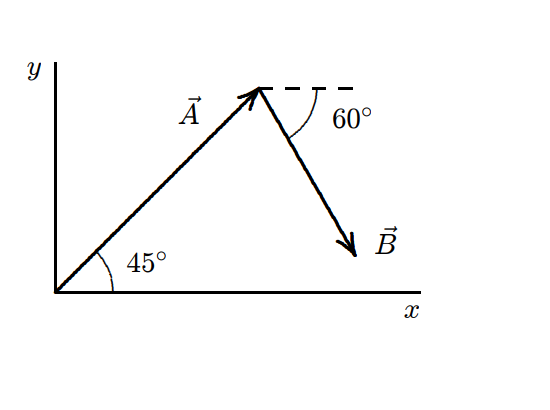
\includegraphics[scale=0.3]{vecs3.png}
					\end{center}
					\question In the diagram above, $\vec{A}$ has magnitude 12 m and $\vec{B}$ has magnitude 8 m. The x component of $\vec{A}$ + $\vec{B}$
					is about: \\
					\begin{oneparchoices}
						\choice 12 m
						\choice 7.2 m
						\choice 19 m
						\choice 20 m
						\choice 18 m
					\end{oneparchoices}
					\textbf{Answer: A}
					\question If the magnitude of the sum of two vectors is less than the magnitude of either vector, then which of the following is necessarily true?
					\begin{choices}
						\choice The scalar product of the vectors must be negative
						\choice The scalar product of the vectors must be positive
						\choice The vectors must be parallel and in opposite directions
						\choice The vectors must be parallel and in the same direction
						\choice None of the above
					\end{choices}
					\textbf{Answer: A}
					\question Let $\vec{R}$ = $\vec{S}\times\vec{T}$ and $\theta\neq90^\circ$, where $\theta$ is the angle between $\vec{S}\text{ and }\vec{T}$ when they are drawn with their tails at the same point. Which of the following is NOT true? \\
					\begin{oneparchoices}
						\choice $\vec{R}=|\vec{S}||\vec{T}|\sin\theta$
						\choice $-\vec{R}=\vec{T}\times\vec{S}$
						\choice $\vec{R}\cdot\vec{S}=0$
						\choice $\vec{R}\cdot\vec{T}=0$
						\choice $\vec{S}\cdot\vec{T}=0$
					\end{oneparchoices} 
					\\ \textbf{Answer: E}
					\question Which of the following quantities is necessarily a fixed vector? \\
					\begin{oneparchoices}
						\choice Velocity vector
						\choice Current density vector
						\choice Position vector
						\choice Momentum vector
						\choice None of the above
					\end{oneparchoices}
					\textbf{Answer: C}
					\question Which of the following unit vectors are perpendicular to both $\hat{i}+2\hat{j}+\hat{k}$ and $3\hat{i}-4\hat{j}+2\hat{k}$
					\begin{oneparchoices}
						\choice $\pm\dfrac{\sqrt{165}}{165}(6\hat{i}+\hat{j}-9\hat{k})$
						\choice $\pm\dfrac{\sqrt{165}}{165}(4\hat{i}+\hat{j}-5\hat{k})$
						\choice $\pm\dfrac{\sqrt{165}}{165}(8\hat{i}+\hat{j}-10\hat{k})$
						\choice $\pm\dfrac{\sqrt{65}}{65}(5\hat{i}+\hat{j}-10\hat{k})$
						\choice None of the above
					\end{oneparchoices}
					\\ \textbf{Answer: C}
					\question Three vectors $\vec{A}$, $\vec{B}$, and $\vec{C}$ lie on the same plane. Which of the following is necessarily true?
					\begin{oneparchoices}
						\choice $\vec{A}\times\vec{B}\times\vec{C}=0$
						\choice $\vec{A}\times\vec{B}=\vec{C}$
						\choice $\vec{A}+\vec{B}+\vec{C}=0$
						\choice $(\vec{C}\times\vec{A})\cdot\vec{B}=0$
						\choice None of the above
					\end{oneparchoices} 
					\\ \textbf{Answer: D}
					\question What is the value of $\alpha$ for which (5$\hat{i}$ - 2$\alpha$$\hat{j}$ + 2$\hat{k}$) is perpendicular to the vector ($\hat{i}$ - $\hat{j}$)? \\
					\begin{oneparchoices}
						\choice $\dfrac{-2}{5}$
						\choice $\dfrac{-5}{2}$
						\choice $\dfrac{2}{5}$
						\choice $\dfrac{5}{2}$
						\choice None of the above
					\end{oneparchoices} 
					\textbf{Answer: B}
					\question Which of the following statements is true?
					\begin{choices}
						\choice If two vectors $\vec{A}$ and $\vec{B}$ lie on two parallel lines, then $\vec{A}\cdot\vec{B}=|\vec{A}||\vec{B}|$
						\choice If the $\vec{A}\cdot\vec{B}=0$, then $|\vec{A}|=0$ or $|\vec{B}|=0$
						\choice The cross product of a vector with itself is equal to the
						square of the same vector. 
						\choice If the dot product of two vectors is maximum, they must be perpendicular.
						\choice None of the above.
					\end{choices}
					\textbf{Answer: E}
					\question The polar expression for a curve is $r=1$, which of the following is true?
					\begin{choices}
						\choice The curve is an equilateral triangle with all side lengths of 2.
						\choice The curve is a unit circle centered at any point in the Cartesian plane.
						\choice The curve is a vertical ellipse with eccentricity of $0.8$.
						\choice The curve is a horizontal ellipse with eccentricity of $1$.
						\choice None of the above.
					\end{choices}
					\textbf{Answer: D}
					\question For what values of x is the vector $x\hat{i} +3\hat{j}+\hat{k}$ is perpendicular to the vector $x\hat{i} – 3x\hat{j}+ 20\hat{k}$? \\
					\begin{oneparchoices}
						\choice $x={1,10}$
						\choice $x={4,5}$
						\choice $x={0}$
						\choice $x={1,10,90}$
						\choice None of the above.
					\end{oneparchoices}
					\\ \textbf{Answer: B}
					\question Vector $\vec{A}$ extends from the origin to a point having polar coordinates $(7, 70^\circ)$ and vector $\vec{B}$ extends from the origin to a point having polar coordinates $(4, 130^\circ)$. What is the value of $\vec{A}\cdot\vec{B}$? \\
					\begin{oneparchoices}
						\choice 30
						\choice 28
						\choice 14
						\choice 50
						\choice None of the above.
					\end{oneparchoices}
					\\ \textbf{Answer: C}
					\question When the following equation is converted into its polar form, which one does it become?
					$$\frac{{4x}}{{3{x^2} + 3{y^2}}} = 6 - xy$$
					\begin{oneparchoices}
						\choice $\dfrac{{4\cos \theta }}{{3r}} = 6 - {r^2}\cos \theta \sin \theta$
						\choice $\dfrac{{6\cos \theta }}{{2r}} = 6 - {r^2}\tan \theta$
						\choice $\dfrac{{4\cos \theta }}{{3r}} = 1$
						\choice $r^3=1$
					\end{oneparchoices}
					\textbf{Answer: A}
					\question An electron, which is a lepton, participates in which of the following interactions?\\
					\begin{oneparchoices}
						\choice Strong and Gravitational
						\choice Strong and Weak
						\choice Electromagnetic and Gravitational \\
						\choice Electromagnetic, Gravitational, and Weak
						\choice Electromagnetic, Gravitational, and Strong 
					\end{oneparchoices}
					\\ \textbf{Answer: D}
					\question A down quark can be changed into an up quark (plus other particles perhaps) by which of the following interactions? \\ 
					\begin{oneparchoices}
						\choice Gravity
						\choice Weak interaction
						\choice Strong interaction
						\choice Electromagnetic interaction
						\choice None of the above
					\end{oneparchoices}
					\\ \textbf{Answer: B}
					\question $\pi^+$ represents a pion (a meson), $\mu^-$ represents a muon (a lepton), $\nu_e$ represents an electron
					neutrino (a lepton), $\nu_\mu$ represents a muon neutrino (a lepton) and p represents a proton. Which of the following decays might occur? \\
					\begin{oneparchoices}
						\choice $\pi^+ \rightarrow \mu^-+\nu_\mu$
						\choice $\pi^+ \rightarrow p+\nu_e$
						\choice $\pi^+ \rightarrow \mu^++\bar{\nu}_e$
						\choice $\pi^+ \rightarrow p+\bar{\nu}_\mu$
						\choice $\pi^+ \rightarrow \mu^++\nu_\mu$
					\end{oneparchoices}
					\\ \textbf{Answer: E}
					\question The messenger(force carrier) particles of the strong interaction are called: \\
					\begin{oneparchoices}
						\choice W and Z bosons
						\choice gluons
						\choice photons
						\choice kaons
						\choice gravitons
					\end{oneparchoices}
					\\ \textbf{Answer: B}
					\question Two particles interact to produce only photons, with the original particles disappearing. The particles must have been: \\
					\begin{oneparchoices}
						\choice mesons
						\choice strongly interacting
						\choice leptons \\
						\choice bosons
						\choice a particle, anti-particle pair
					\end{oneparchoices}
					\\ \textbf{Answer: E}
					\question A bus travels 40 kilometers at an average speed of 80 km/h and then travels 40 kilometers at
					an average speed of 40 km/h. The average speed of the car for this 80-km trip is \\
					\begin{oneparchoices}
						\choice 48 km/h
						\choice 53 km/h
						\choice 80 km/h
						\choice 40 km/h
						\choice 45 km/h
					\end{oneparchoices}
					\\ \textbf{Answer: B}
					\question A drag racing car starts from rest at $t = 0$ and moves along a straight line with velocity given by $v = bt^2$, where $b$ is a constant. The expression for the distance traveled by this car from its
					position at $t = 0$ is: \\
					\begin{oneparchoices}
						\choice $2bt$
						\choice $\dfrac{bt^3}{3}$
						\choice $\dfrac{2bt^3}{3}$
						\choice $4bt$
						\choice None of the above
					\end{oneparchoices}
					\\ \textbf{Answer: B}
					\question The position y of a particle moving along the y axis depends on the time $t$ according to the equation $y = at-bt^2$. The dimensions of the quantities a and b are respectively: \\
					\begin{oneparchoices}
						\choice $\dfrac{L^2}{T}$, $\dfrac{L^3}{T^2}$
						\choice $\dfrac{L}{T^2}$, $\dfrac{L^2}{T}$
						\choice $\dfrac{L}{T}$, $\dfrac{L}{T^2}$
						\choice $\dfrac{L^3}{T}$, $\dfrac{T^2}{L}$
						\choice None of the above
					\end{oneparchoices}
					\\ \textbf{Answer: C}
					\question At time t = 0, a car has a velocity of 16 m/s. It slows down with an acceleration given by
					$a(t)=-0.50t$, in $m/s^2$ for t in seconds. At the end of 4.0 s, it has traveled:\\
					\begin{oneparchoices}
						\choice 14 m
						\choice 25 m
						\choice 2 m
						\choice 59 m
						\choice None of the above
					\end{oneparchoices}
					\\ \textbf{Answer: D}
					\question The average speed of a moving object during a given interval of time is always:
					\begin{choices}
						\choice the magnitude of its average velocity over the interval
						\choice the distance covered during the time interval divided by the time interval
						\choice one-half its speed at the end of the interval
						\choice its acceleration multiplied by the time interval
						\choice one-half its acceleration multiplied by the time interval.
					\end{choices}
					\textbf{Answer: B}
					\subsection*{Free Response Problems}
					\question[1] Out of the 4 fundamental interactions, state which ones neutrinos interact through. Explain why neutrinos are ironically perfect for astronomy. \vspace{1.5in}
					\question[1] Given the points O(0, 0, 0), P(1, 2, 3), Q(1, 1, 2), R(2, 1,1), find the volume of the parallelepiped with edges $\overrightarrow{OP}$, $\overrightarrow{OQ}$, and $\overrightarrow{OR}$.\vspace{1.5in}
					\question[1] Find a vector $\vec{u}$ with its given magnitude and that satisfies the following conditions 3 conditions.
					\begin{itemize}
						\item $\vec b=(2\sin t)\hat{i}+(2\cos t)\hat{j}+\hat{k}$
						\item $|\vec u|=2$ 
						\item $\vec{u}$ and $\vec{b}$ are anti-parallel.
					\end{itemize}
					\vspace{1.4in}
					\question[1] Starting at time $t = 0$, an object moves along a straight line. Its coordinate in meters is given by $x(t) = 75t-1.0t+3$, where $t$ is in seconds. What is the acceleration of this object when it momentarily stops?\vspace{1.5in}
					\question[1] Two automobiles are 180 kilometers apart and traveling toward each other. One automobile is moving at 50 km/h and the other is moving at 40 km/h. In how many hours will they meet?\vspace{2.5in}
					\question[2] Starting at time $t = 0$, an object moves along a straight line with velocity in $m/s$ given by $v(t) = 98-3t^2$, where t is in seconds. At $t=0$, the object was at a position, $s(0)=-28$. What are the position and acceleration of this object when it momentarily comes to rest.\vspace{1.5in}
					\question[1] What is the acceleration of a car that moves at a steady velocity of 100 km/h for 100 seconds?\vspace{1in}
					\question[1] Is it possible for a helicopter to have an acceleration due east and a velocity due west? If so, what would be going on? If not, why not?\vspace{1in}
					\question[1] What is the value of $\hat{i}\cdot(\hat{j}\times\hat{k})$?\vspace{1.3in}
				\end{questions}
			\end{document}